\documentclass{beamer}
% Make sure to run this file with PDFLatex.
%%%%%%%%%%%%%%%%%%%%%%%%%%%%%
% Do not change the next few lines
\usepackage{beamerthemesplit}
\usepackage[english]{babel}

% T1 encoding with Latin Modern provides typewriter braces for \{...\}
% in Twelf code and a bold italic sans font for \emph
\usepackage[T1]{fontenc}
\usepackage{lmodern}

% Stop TOC from appearing at top of every slide
\setbeamertemplate{headline}{}

% Make item symbol square
\setbeamertemplate{itemize item}[square]


% Input my macros
\usepackage{graphicx}

% AMS macros (\text, symbols)
\usepackage{amsmath}
\usepackage{amssymb}

% Packages for formatting code segments
\usepackage{verbatim}
\usepackage{alltt}

% Packages for proof trees
\usepackage{proof}

% Adding line space
\newcommand{\linespace}{\vspace{\baselineskip}}

% context-free grammars
\newcommand{\bnfdef}{\mathrel{\colon\colon\mathord{=}}}
\newcommand{\bnfalt}{\mathrel{\mid}}

% Small typewriter text for inline Twelf code; \text makes it work in math
\newcommand{\code}[1]{\text{\small\texttt{#1}}}

% Emphasize code or math
\newcommand{\cemph}[1]{\textcolor{red}{#1}}

% For highlighting ground Twelf terms,
% which are terms allowed to be universally quantified inputs,
% existentially quantified, or constants
\newcommand{\gtrm}[1]{\textcolor{blue}{#1}}

% For highlighting un-ground Twelf terms
\newcommand{\utrm}[1]{\textcolor{orange}{#1}}

\newcommand{\gtrmbig}[1]{\gtrm{{\Large #1}}}
\newcommand{\utrmbig}[1]{\utrm{{\Large #1}}}

\let\OldInfer\infer
\renewcommand{\infer}[3][]
{\OldInfer[\text{\scriptsize\texttt{#1}}]{#2}{#3}}

\newcommand{\cinfer}[3][]{\infer[#1]{\code{#2}}{#3}}
\newcommand{\ttinfer}[3][]{\infer[#1]{\texttt{#2}}{#3}}
\newcommand{\stepto}{\mapsto}


\renewcommand{\emph}[1]{\textbf{\textit{#1}}}

% Now Start entering your information.
%\title{Taming the Wildcards: \\
% Combining Definition- and Use-Site Variance}
% \title{Taming the Wildcards}

\title[Twelf Tutorial\hspace{2em}\insertframenumber/
\inserttotalframenumber]{Twelf Tutorial}

\subtitle{Twelf Encoding of MiniLang}

\author[John Altidor]{\textbf{John Altidor}}
\date{}
% \institute{Logic Seminar}

% PDF document properties; Beamer sets the title and author itself
\hypersetup{
  pdfsubject={Tutorial on the Twelf proof assistant and the Twelf encoding of MiniLang},
  pdfkeywords={Twelf, LF, proof assistant, logical framework, higher-order abstract syntax, type safety, preservation, MiniLang, formal verification}
}

\begin{document}
\frame{\titlepage}

\section{Motivation}

\begin{frame}{Motivation}
\begin{itemize}
\item Proving language properties is important.
	\begin{itemize}
  \item Rule out certain errors (e.g., assuming
  wrong number of bytes for an object).
  \item Well-defined behavior throughout execution
  (e.g., no segmentation fault or accessing wrong
  parts of memory).
  \item Publishing.
  \end{itemize}

\pause
\item But proofs are long, error-prone, and difficult
to validate.
	 \begin{itemize}
	 \item \emph{+20 pages} is common for a type safety proof.
	 \end{itemize}
\end{itemize}
\end{frame}

\begin{frame}{Typical Proof Structure}
\begin{itemize}
\item Example taken from type soundness proof of TameFJ
calculus \\
{\scriptsize (Cameron, Drossopoulou, and Ernst,
\textit{A Model for Java with Wildcards}, ECOOP 2008).}
\end{itemize}
\begin{center}
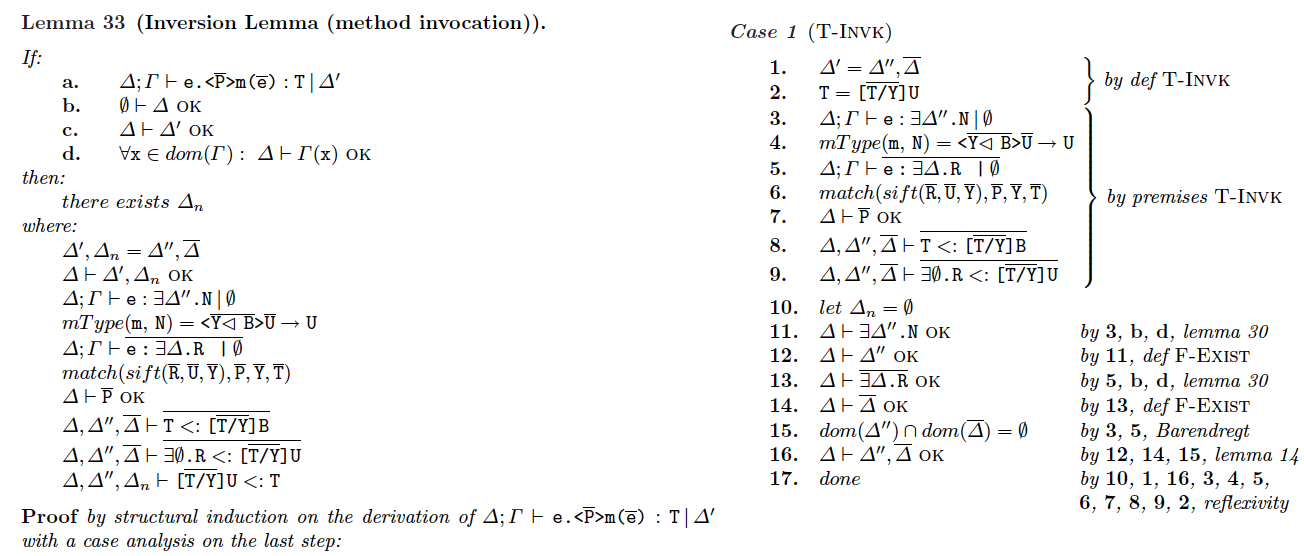
\includegraphics[width=\textwidth,keepaspectratio]{tamefj_lemma.png}
\end{center}
\begin{itemize}
\item Lots of steps, lemmas, and opportunities for errors
in proofs of language properties.
\end{itemize}
\end{frame}

\section{Introduction to Proof Assistants}

\begin{frame}{What is a Proof Assistant}
Multiple ways of proving theorems with a computer:
\begin{itemize}
\item \emph{Automatic theorem provers} find complete proofs
on their own.
  \begin{itemize}
  \item Not all proofs can be derived automatically.
  \end{itemize}
\pause
\item \emph{Proof checkers} simply verify the proofs they
are given.
  \begin{itemize}
  \item These proofs must be specified in an extremely
  detailed, low-level form.
  \end{itemize}
\pause
\item \emph{Proof assistants} are a hybrid of both.
  \begin{itemize}
  \item ``Hard steps'' of proofs (the ones requiring deep insight)
  are provided by a human.
  \item ``Easy steps'' of proofs can be filled in automatically.
  \end{itemize}
\item (above bullet points taken from UPenn's Software Foundations
course slides)
\end{itemize}
\end{frame}

\begin{frame}{Twelf Proof Assistant}
\begin{center}

\includegraphics[width=0.26\textwidth,keepaspectratio]{mediumelf.png}
\end{center}

\begin{itemize}
\item Automated support for \emph{deriving proofs} and
\emph{checking proofs} of language properties.

\item Implementation of the LF calculus \\
(calculus for reasoning about deductive systems).

\item Alternatives: Rocq (formerly Coq), Isabelle, Agda, etc.

\item Presenting Example Twelf Encoding of MiniLang.
\end{itemize}
\end{frame}

\section{Constructive Logic}

\begin{frame}{Constructive Logic}
\begin{itemize}
\item Twelf is a \emph{constructive} (not classical)
proof assistant.
\item Proposition is true \emph{iff} there exists a proof
of it.
\item Law of excluded middle not assumed:  $P \lor \neg P$.
  \begin{itemize}
  \item Proving $P \lor \neg P$ \emph{requires} either:
    \begin{itemize}
    \item Proof of $P$ \emph{OR} Proof of $\neg P$.
    \end{itemize}
\pause
  \item No case-split on undecidable propositions. Not allowed:
    \begin{itemize}
    \item \cemph{If \textit{halts(TuringMachine)}}
      then proof of $A$ else proof of $B$.
    \end{itemize}
  \end{itemize}
\pause
\item No choice or description operators
 (e.g., Hilbert's choice operator \cemph{$\epsilon x . P(x)$}).
  \begin{itemize}
  \item $\ln(x) = u$ such that $x = e^u$.
  \item Definition in Isabelle/HOL with description operator \texttt{THE}: \\
    \texttt{definition ln ::\ real => real where} \\
    \texttt{ln x = \cemph{THE u}.\ exp u = x}.
  \end{itemize}
\pause
\item In Twelf: Writing a proof = Writing a program.
	\begin{itemize}
	\item Proofs are programs.
	\end{itemize}
\end{itemize}
\end{frame}

\section{Introduction to Twelf}

\begin{frame}{Running Twelf}
\begin{itemize}
\item Lecture will involve in-class exercises.
\item Download Twelf:
\end{itemize}
\begin{center}
\begin{Large}
\cemph{\url{https://twelf.org/download/}}
\end{Large}
\end{center}
\begin{itemize}
\item Code of the examples, with a Docker image for running
Twelf without installing it: \\
\url{https://github.com/jgaltidor/twelf_tutorial}
\end{itemize}
\end{frame}

\begin{frame}{Kinds: Category of Types}
\begin{itemize}
\item
Three \emph{levels} of objects in Twelf:
  \begin{itemize}
  \item \emph{Kinds} are at highest level.
  \item \emph{Types} are at second level.
  \item \emph{Terms} are at lowest level.
  \end{itemize}

\pause
\item Each type is of a certain kind. \\
(Twelf syntax: ``\code{someType : someKind}'')
\item Each term is of a certain type. \\
(Twelf syntax: ``\code{someTerm : someType}'')
\item Twelf overloads language constructs with same syntax. \\
(elegant but confusing too)

\pause
\item Contrived examples:
  \begin{itemize}
  \item Term \code{[1, 2, 3]} is of type \code{ArrayInt}.
  \item Type \code{ArrayInt} is of kind \code{\cemph{type}}.
  \end{itemize}

\pause
\item The kind \code{\cemph{type}} is a predefined kind in Twelf: \\
the kind of ordinary types.
\end{itemize}
\end{frame}

\section{Functions}

\begin{frame}{Functions}
\begin{itemize}
\item Twelf supports defining functions: \\
\code{int : type.} \; \code{one : int.} \\
\code{\cemph{plusOne : int -> int}.}

  \begin{itemize}
  \item \code{plusOne} is a \emph{function term}.
  \item \code{plusOne} takes in a term of type \code{int}
  and returns a term of type \code{int}.
  \item The type of function term \code{plusOne} is
  \code{int -> int}.
  \item \code{\cemph{(plusOne one)}} has type \code{int}.
  \end{itemize}

\pause
\item Functions taking in \emph{multiple} arguments
are represented using their \emph{curried form}:

\item \code{\cemph{plus: int -> int -> int}.}

  \begin{itemize}
  \item \code{int -> int -> int} is curried form
  of \code{(int, int) -> int}.
  \item \code{int -> int -> int} = \code{int -> (int -> int)}.
  \item \code{(plus one)} has type \code{int -> int}.
  \item \code{(plus one one)} has type \code{int}.
  \end{itemize}
\end{itemize}
\end{frame}

\begin{frame}{Functions Returning Types}
\begin{itemize}
\item Recall that \code{\cemph{type}} is a \emph{kind} (type of types).

\item Functions can also return \emph{types}:

\item \code{equalsOne : int -> \cemph{type}.}

  \begin{itemize}
  \item \code{equalsOne} is a function \emph{term}.
  \item \code{equalsOne} takes in a term of type \code{int}
  and returns a \emph{type} of kind \code{type}.
  \item The type of function term \code{equalsOne} is
  \code{int -> type}.
  \item \code{\cemph{(equalsOne one)}} is a \emph{type} of
  kind \cemph{type}.
  \end{itemize}

\pause
\item \code{\cemph{oneIsOne : (equalsOne one)}.}
  \begin{itemize}
  \item Defines a new \emph{term} \code{oneIsOne} of
  \emph{type} \code{(equalsOne one)}.
  \end{itemize}

\pause
\item A function type is a kind if its return type
is also a kind.
  \begin{itemize}
  \item \code{int -> type} is a kind.
  \item \code{int -> (int -> type)} is a kind.
  \item \code{int -> int -> type} =
        \code{int -> (int -> type)} is a kind.
  \end{itemize}
\item \code{\cemph{type}} is \emph{not} allowed on the left-hand side of arrow (\code{->}).
\end{itemize}
\end{frame}

\section{MiniLang Syntax}

\begin{frame}{MiniLang Syntax in Twelf}
\begin{itemize}
\item The object language is MiniLang (the object of study).
\item Syntactic categories encoded w/ object types
(defined types).
  \begin{itemize}
  \item \texttt{\cemph{exp : type.}}
  \item Defines type \texttt{\cemph{exp}} of kind \texttt{\cemph{type}}.
  \item \texttt{\cemph{exp}} represents syntactic category $e$.
  \item Terms in the grammar of $e$ have type \texttt{\cemph{exp}}.
  \end{itemize}

\pause
\item Grammar productions encoded w/ \emph{functions} between
syntactic categories.
  \begin{itemize}
  \item \cemph{\texttt{add : exp -> exp -> exp.}}
  \item $\mathit{Expression} \; e \; \bnfdef \; \code{+($e_1$; $e_2$)}$
  \item \code{add} takes in \emph{two} arguments.
  \item \code{exp -> exp -> exp} is curried form of \code{(exp, exp) -> exp}.
  \end{itemize}
\end{itemize}
\end{frame}


\section{Higher-Order Abstract Syntax}

\begin{frame}{Terms w/ Variables Using Higher-Order Abstract Syntax (HOAS)}
\begin{itemize}
\item Abstract syntax from earlier slides is
\emph{first-order abstract syntax (FOAS)}.
  \begin{itemize}
  \item Each AST has form $o(t_1, t_2, \ldots, t_n)$,
  where $o$ is operator and $t_1, \ldots, t_n$ are ASTs.
  Example:
\pause
    \begin{itemize}
    \item \code{+(num[3]; num[4])}
    \item \code{add (enat 3) (enat 4)}
    \end{itemize}
  \end{itemize}

\pause
\item ASTs in \emph{Higher-Order Abstract Syntax (HOAS)}:
\item Each $t_i$ in $o(t_1, t_2, \ldots, t_n)$ has form:
\[ \cemph{x_1, x_2, \ldots, x_k.t} \]
\item $t$ is a FO-AST.
\item Each $x_j$ is a variable bound in $t$.
\item $k \geq 0$; if $k = 0$, then no variable is declared.
\end{itemize}
\end{frame}


\begin{frame}{HOAS Encoding of \texttt{let} Expression}
\begin{itemize}
\item First, \code{let} expression in FOAS:
\[ \code{let($x$; $e_1$; $e_2$)} \]

\pause
\item \code{let} expression in HOAS:
\[ \code{let($e_1$; \cemph{$x.e_2$})} \]
\item ``$x.e_2$'' captures that $x$ is bound in $e_2$.

\pause
\item HOAS lets us know where variables are being bound.
\[ \code{let(3; \cemph{$x$.+($x$; 4)})} \equiv \code{let(3; \cemph{$y$.+($y$; 4)})}\]
\item The two terms above are \emph{alpha-equivalent}.
\end{itemize}
\end{frame}


\begin{frame}{Higher-Order Terms are Functions}
\begin{itemize}
\item Functions are really terms with \emph{holes}/unknowns:
($3 + \bullet$).

\pause
\item Holes are represented by \emph{variables}.
\item Holes filled in by \emph{applying} (terms w/ holes)/functions.
\item Holes \emph{abstract} details.

\pause
\item ``$x.e$'' represented by \emph{lambda abstraction}
      ``$\cemph{\lambda x:\tau.e}$''.
\item Twelf's syntax of ``$\lambda x:\tau.e$'':
      ``\texttt{\cemph{[$x : \tau$] $e$}}''
\end{itemize}
\end{frame}


\begin{frame}{\texttt{let} expression in Twelf HOAS}
\begin{itemize}
\item Twelf type signature of \code{let}:
\[ \texttt{let : exp -> $\underbrace{\texttt{\cemph{(exp -> exp)}}}_{x.e_2}$ -> exp.} \]

\pause
\item Example HOAS term in Twelf:

\begin{center}
\resizebox{\linewidth}{!}{%
\begin{tabular}{l|l}
\textit{Concrete Syntax} & \textit{Twelf HOAS} \\ \hline
\code{let x be $\underbrace{\code{1 + 2}}_{e_1}$ in
                $\underbrace{\code{x + 3}}_{e_2}$} &
  \code{let $\underbrace{\code{(add 1 2)}}_{e_1}$
    $\underbrace{\cemph{\code{([x:exp] add x 3)}}}_{x.e_2}$}
\end{tabular}}
\end{center}

\pause
\item No need to define object (MiniLang) variables.
\item \emph{LF variables} remove need for object variables.
\item No need to define substitution (nor requisite theorems)
as well.
\end{itemize}
\end{frame}


\section{Predicates}

\begin{frame}{Predicates in Twelf}
\begin{itemize}
\item Predicates are defined with \emph{type families}: \\
Functions that return types (not terms).

\item Typing Predicate:  $e : \tau$

\item Twelf Encoding:
\cemph{\texttt{of : exp -> typ -> type.}}

\pause
\item Type families return \emph{dependent types}.
	\begin{itemize}
	\item Types that contain terms (or \emph{depend on} terms).
	\end{itemize}

\pause
\item Examples:
  \begin{itemize}
  \item \texttt{3} is a \emph{term} of type \emph{nat}.
\pause
  \item Let \texttt{Vec} be a function that given \emph{nat} $n$,
  \texttt{Vec($n$)} returns the type of $n$-dimensional vectors.
\pause
  \item \texttt{Vec(3)} is a \emph{dependent type} representing
  3-dimensional vectors.
\pause
  \item \texttt{[4, 1, 3]} is a \emph{term} of \emph{type} \texttt{Vec(3)}.
\pause
  \item \texttt{Vec} is a \emph{type family} because it is a
  function that returns dependent types.
  \end{itemize}
\end{itemize}
\end{frame}


\begin{frame}{Judgments are Dependent Types}
\begin{itemize}

\item Judgments/Propositions (instantiations of predicates) represented
by dependent types.

\item Judgment $\cemph{z : \texttt{num}}$ represented by type
\texttt{\cemph{(of (enat z) num)}}.

\item Dependent type \texttt{(of $e$ $\tau$)} represents
judgment ``$e : \tau$''.

\pause
\item \emph{Derivation/Proof} of ``$e : \tau$'' represented
by \emph{term} of type \texttt{(of $e$ $\tau$)}.

\pause
\item Curry-Howard Correspondence: \\
\emph{Proofs} are terms. \\
\emph{Propositions/Judgments} are types.

\end{itemize}
\end{frame}


\begin{frame}{Pi-Abstractions}
\begin{itemize}
\item  Function/\emph{Lambda Abstraction} ``$\lambda x:S.e$'' of type
$\cemph{S \rightarrow T}$:
  \begin{itemize}
  \item Takes in a term $s$ of type $S$.
  \item Returns a term of type $T$.
  \end{itemize}

\pause
\item Function/\emph{Pi-abstraction} of type pi-type $\cemph{\Pi x:S.T}$:
  \begin{itemize}
  \item Takes in a term $s$ of type $S$.
  \item Returns a term of type \cemph{$[s / x]T$}.
  \end{itemize}

\pause
\item If $x \notin \mathit{fv}(T)$, then $\Pi x:S.T \equiv S \rightarrow T$.

\pause
\item If $x \in \mathit{fv}(T)$, then $\Pi x:S.T$ returns term of a
dependent type.

\pause
\item Twelf Syntax for $S \rightarrow T$: \\
\texttt{S -> T}

\pause
\item Twelf Syntax for $\Pi x:S.T$: \\
\cemph{\texttt{\{x:S\} T}}
\end{itemize}
\end{frame}

\begin{frame}{Inference Rules are Functions}
\[ \cinfer[T.1]{num[$n$] : num}{ } \]

\begin{itemize}
\item
\cemph{\texttt{of/nat : \{N:nat\} of (enat N) num.}}
\item Twelf Convention:
  \begin{itemize}
  \item Constants start with lowercase letters.
  \item Variables/parameters start with uppercase letters.
  \end{itemize}

\pause
\item \texttt{(of/nat z) $\neq$ (of (enat z) num)}.
\item Function \texttt{of/nat} \emph{returns terms} not types.
\item Function \texttt{of} \emph{returns types}.

\pause
\item \texttt{(of/nat z)} $=$ \emph{term} of type \texttt{(of (enat z) num)}.
  \begin{itemize}
  \item Example legal assignment: \\
        \texttt{y : (of (enat z) num) = (of/nat z).}
  \end{itemize}

\pause
\item \texttt{(of/nat z)} is a \emph{derivation/term} of judgment
$z : \texttt{num}$ represented by type \texttt{(of (enat z) num)}.
\end{itemize}
\end{frame}


\begin{frame}{Premises are Inputs}
\[
\cinfer[T.4]{+($e_1$; $e_2$): num}
  {\code{$e_1$: num} & \code{$e_2$: num}}
\]
\begin{itemize}
\item Twelf Encoding: \\
\texttt{of/add : of (add E1 E2) num} \\
$\qquad$ \texttt{<- \cemph{of E1 num}} \\
$\qquad$ \texttt{<- \cemph{of E2 num}.}

\item Given a proof of \texttt{(of E2 num)} \emph{and}
\item Given a proof of \texttt{(of E1 num)}
\item \texttt{of/add} returns proof of
\texttt{(of (add E1 E2) num)}

\end{itemize}
\end{frame}


\begin{frame}{Implicit and Explicit Parameters}
\begin{itemize}
\item \texttt{of/nat: \{\cemph{N:nat}\} of (enat \cemph{N}) num.}

\item Parameter \texttt{\cemph{N}} is \emph{explicit}
in the above signature.
\item Explicit parameters \emph{must be specified} in
function applications.

\item \texttt{D : of (enat z) num = of/nat \cemph{z}.}
\end{itemize}

\pause
\begin{itemize}
\item \texttt{of/nat: of (enat \cemph{N}) num.}
\item Parameter \texttt{\cemph{N}} is \emph{implicit}
in the above signature.
\item Implicit parameters \emph{cannot be specified}
by programmer in function applications.
\item \texttt{D : of (enat \cemph{z}) num = of/nat.}
\item Twelf figures out from the context
(type of left-hand side of assignment)
that \texttt{\cemph{z}} is the implicit parameter that
\texttt{of/nat} should be applied to.
\end{itemize}
\end{frame}


\section{Logic}

\begin{frame}{First-Order Quantification Only}
\begin{itemize}
\item Can only quantify over \cemph{first-order} terms.
\item \emph{Allowed}:
	\begin{itemize}
	\item \texttt{add : exp -> exp -> exp.}
	\item \texttt{let : exp -> (exp -> exp) -> exp.}
	  \begin{itemize}
	  \item A \emph{higher-order term} is a function,
	  where one of its inputs is also a function.
	  \end{itemize}
	\end{itemize}

\pause
\item \emph{Not allowed}:
	\begin{itemize}
  \item \texttt{quantifyTypes : exp -> \code{\cemph{type}} -> exp.}
	\item \texttt{allIsTrue : \{Prop:\cemph{type}\} Prop.}
	\end{itemize}

\item The kind \texttt{\cemph{type}} categorizes Twelf types.

\pause
\item No type polymorphism implies no \emph{general} logical connectives.
\item \emph{Not allowed}: \\
\texttt{conjunction :} \\
\texttt{\cemph{\{P:type\} \{Q:type\}} P -> Q -> (and P Q)}.
\end{itemize}
\end{frame}

\begin{frame}{Predicativity}
\begin{itemize}
\item Different term levels used to restrict quantification.
  \begin{itemize}
  \item Twelf terms are first-order terms; e.g., \texttt{(s z)}.
  \item Twelf types are second-order terms; e.g., \texttt{nat}.
  \item Twelf kinds are third-order terms; e.g., \texttt{type}.
  \end{itemize}

\pause
\item Twelf only allows \emph{predicative} definitions:
  \begin{itemize}
  \item Cannot apply term to itself. (Cannot quantify over oneself.)
  \item No term has itself as type. (Not allowed: \texttt{\cemph{typ :\ typ}}.)
  \item Disallows Russell's paradox: \\
  Let $H = \{ x \; | \; x \notin x\}$.
  Then $\underbrace{\cemph{H \in H \iff H \notin H}}_{\textit{False}}$.
  \end{itemize}

\item Helps Twelf avoid logical inconsistency \\
(i.e., proving false/uninhabited type).

\item False implies any proposition (including false ones).

\item False/uninhabited types used for constructive
proofs by contradiction.
\end{itemize}
\end{frame}

% Hence, second-order predicates (predicates with quantified
% predicates) can't be represented in Twelf naturally.

% Proposition, \forall x. P(x), can be thought of as the
% lambda function, \lambda x. P(x).
% Maybe, in some "extra slides", add a Table mapping
% propositions to types (e.g., and maps to product type)
% such and "and" type requires polymorphism being able to
% quantify over types.
% and inductive type definition (type family) in Coq:
%   Inductive and (A B : Prop) : Prop :=  conj : A -> B -> A /\ B


% Also, False implies any theorem is true.
% To prove:
%   someTheorem : False -> someProp.
%   %mode +F -S
% Since there are no constructors/cases for False,
% then all cases for someTheorem are handled.
% and Twelf can conclude someTheorem is a total
% relation.

\section{Laboratory}

\begin{frame}{Laboratory}
\begin{itemize}
\item Create language of numbers with subtyping in Twelf.
\end{itemize}
\[
\begin{array}{llrl@{\hspace{0.5cm}}l}
\mathbf{Category}   & \mathbf{Item}   & & \mathbf{Abstract} & \mathbf{Concrete} \\
\mathit{Terms}      & e & \bnfdef & \code{zero}                    & 0 \\
                    &   & \bnfalt & \code{pi}                      & \pi \\
                    &   & \bnfalt & \code{img}                     & \sqrt{-1} \\
\mathit{Types}      & t & \bnfdef & \code{number}                  & \textit{num} \\
                    &   & \bnfalt & \code{real}                    & \textit{real} \\
                    &   & \bnfalt & \code{complex}                 & \textit{complex} \\
                    &   & \bnfalt & \code{int}                     & \textit{int}
\end{array}
\]
\end{frame}

\begin{frame}{More Exercises}
\begin{itemize}
\item \emph{Subtyping} Rules (not all):
\[
\infer{\textit{complex} <: \textit{num}}{ }
\qquad
\infer{\textit{real} <: \textit{num}}{ }
\qquad
\infer{\textit{int} <: \textit{real}}{ }
\]
\item \emph{Typing} Rules (not all):
\[
\infer{0 : \textit{int}}{ }
\qquad
\infer{\pi : \textit{real}}{ }
\qquad
\infer{\sqrt{-1} : \textit{complex}}{ }
\]
\item Define \emph{reflexive} and \emph{transitive} rules for subtyping.
\item Define \emph{subsumption} rule for typing judgment.
\item \emph{Prove} $0 : \textit{num}$.
	\begin{itemize}
	\item Fill in the blank below:
	\item \texttt{D : (of zero num) = } $\bullet$
	\end{itemize}
\item Starter file and solution: \\
{\footnotesize \url{https://github.com/jgaltidor/twelf_tutorial/tree/master/exercises/numsubtype}}
\end{itemize}
\end{frame}



\section{Hypothetical Judgments}

\begin{frame}{Hypothetical Judgments in Twelf}
\begin{itemize}
\item What happened to typing context \cemph{$\Gamma$}?

\pause
\item \emph{Hypothetical Judgments}: \\
Judgments made under the assumption of other judgments.

\pause
\item Encoded w/ \emph{higher-order types}: \\
Function types where one of the inputs is also a
function type.

\pause
\item Input function types represent hypothetical assumptions.
\item Similar to higher-order terms. \\
(Another application of HOAS)
\item $\Gamma$ does not need to be defined.
\end{itemize}
\end{frame}


\begin{frame}{Typing \texttt{let} expression in Twelf HOAS}
\[
\cinfer[T.6]{$\Gamma \vdash$ let($x$; $e_1$; $e_2$): $\tau_2$}
  {\Gamma \vdash e_1: \tau_1
   &
   \cemph{\Gamma , x : \tau_1 \vdash e_2 : \tau_2}
  }
\]
\begin{itemize}
\item Twelf Encoding: \\
\texttt{of/let : \cemph{(\{x: exp\} of x T1 -> of (E2 x) T2)} ->} \\
$\qquad$ \texttt{of E1 T1 ->} \\
$\qquad$ \texttt{of (let E1 ([x] E2 x)) T2.}

\pause
\item First, a Twelf \emph{coding convention}: \\
Return type \texttt{(of (let E1 \cemph{([x] E2 x)}) T2)}
could be replaced with
\texttt{(of (let E1 \cemph{E2}) T2)}.

\item \texttt{E2} in both cases is of type \texttt{(exp -> exp)}.

\item \texttt{([x] E2 x)} used for readability: \# of inputs explicit.

\item \texttt{([x] E2 x)} is called the \emph{eta-expansion}
of \texttt{E2}.

\end{itemize}
\end{frame}


\begin{frame}{\texttt{of/let}'s first input type}
\begin{itemize}
\item
Let $f$ be a function of \texttt{of/let}'s first input type: \\
\cemph{\texttt{(\{x: exp\} of x T1 -> of (E2 x) T2)}}.

\item That type models hypothetical judgment:
$\cemph{\Gamma , x : \tau_1 \vdash e_2 : \tau_2}$.

\pause
\item $f$'s first input is an \texttt{exp} term bound to LF variable \texttt{x}.
\pause
\item $f$'s second input is a term \texttt{\cemph{dx}} of type \texttt{(of x T1)}. \\
\texttt{\cemph{dx}} = proof that $f$'s first input has type \texttt{T1}
\pause
\item $f$'s output is a term of type \texttt{(of (E2 x) T2)}: \\
a proof that \texttt{E2} instantiated with \texttt{exp} term
\texttt{x} has type \texttt{T2}.

\pause
\item \texttt{\cemph{dx}} of type \texttt{(of x T1)} can be
\emph{used in the definition of} $f$
to return a proof/term of type \texttt{(of (E2 x) T2)}.

\item The ability to use a proof (\texttt{\cemph{dx}}) of type
\texttt{(of x T1)} to derive a proof of type \texttt{(of (E2 x) T2)}
simulates the ability to use an assumption $x : \tau_1$ to prove $e_2 : \tau_2$.
\end{itemize}
\end{frame}


\begin{frame}[containsverbatim]{Exercise Applying Hypothetical Judgment}
\begin{itemize}
\item Derive the judgment
$\cemph{\vdash \texttt{let x be 1 in x + 0} : \code{num}}$
in Twelf.

\item Twelf encoding of above judgment: \\
\code{\cemph{of (let (enat (s z)) ([x:exp] add x (enat z))) num}.}

\item Recall important signatures (displaying implicit parameters):

\begin{verbatim}
of/let :
  {T1:typ} {E2:exp -> exp} {T2:typ} {E1:exp}
    ({x:exp} of x T1 -> of (E2 x) T2) -> of E1 T1
      -> of (let E1 ([x:exp] E2 x)) T2.

of/nat : {N:nat} of (enat N) num.

of/add : {E2:exp} {E1:exp}
  of E2 num -> of E1 num -> of (add E1 E2) num.
\end{verbatim}

\end{itemize}
\end{frame}

\begin{frame}[containsverbatim]{Solution to Previous Exercise}
\begin{itemize}
\item Derive the judgment
$\cemph{\vdash \texttt{let x be 1 in x + 0} : \code{num}}$
in Twelf.

\item Twelf encoding of above judgment: \\
\code{\cemph{of (let (enat (s z)) ([x:exp] add x (enat z))) num}.}

\item Recall important signatures (without implicit parameters):

\begin{verbatim}
of/let : ({x:exp} of x T1 -> of (E2 x) T2) ->
  of E1 T1 -> of (let E1 ([x:exp] E2 x)) T2.
of/nat : of (enat N) num.
of/add :
  of E2 num -> of E1 num -> of (add E1 E2) num.
\end{verbatim}

\item Twelf proof of above judgment:

\begin{alltt}
of/let
  ([x:exp] [\cemph{dx:of x num}] of/add of/nat \cemph{dx})
  of/nat
\end{alltt}
\end{itemize}
\end{frame}


\section{Modes}

\begin{frame}{Relations w/ Inputs and Outputs (Modes)}
\begin{itemize}
\item Inputs/Outputs defined with \texttt{\cemph{\%mode}}
declaration. \\

\texttt{of : exp -> typ -> type.} \\
\texttt{\cemph{\%mode of +E -T}.}

\item Inputs marked with \texttt{\cemph{+}}.
\item Outputs marked with \texttt{\cemph{-}}.

\pause
\item
Outputs can be derived automatically
using Twelf's logic programming engine
(example later).

\pause
\item
Not all relations require modes.

\item
Modes are necessary for \emph{specifying theorems}.

\item
Modes used also for \emph{checking proofs of theorems}.

\pause
\item
Only \emph{ground} terms may be applied to relations
w/ modes in rules (details later).
\end{itemize}
\end{frame}


\begin{frame}{Backward Arrow vs. Forward Arrow}
\begin{itemize}
\item Output terms must be \emph{ground} given
ground input terms.
  \begin{itemize}
  \item Ground terms do not contain \emph{free} variables.
  \item Output terms are fixed (ground) wrt (ground) inputs.
  \end{itemize}

\item Forward ``\texttt{\cemph{->}}'' reflects
\emph{order that premises are passed to rules/functions}
and makes proofs more natural.

\item Backward ``\texttt{\cemph{<-}}'' reflects
\emph{order of resolving ground terms}.

\pause
\item \emph{Order of args} allowed by Twelf: \\
\texttt{of/let : (\{x: exp\} of x T1 -> of (E2 x) T2) ->} \\
$\qquad$ \texttt{of E1 T1 ->} \\
$\qquad$ \texttt{of (let E1 ([x] E2 x)) T2.}

\pause
\item Order of args that \emph{causes error}: \\
\texttt{of/let : \cemph{of E1 T1} ->} \\
$\qquad$ \texttt{\cemph{(\{x: exp\} of x T1 -> of (E2 x) T2)} ->} \\
$\qquad$ \texttt{of (let E1 ([x] E2 x)) T2.}

\pause
\item Error message:
\texttt{Occurrence of variable T1 in output (-) argument
\cemph{not necessarily ground}}
\end{itemize}
\end{frame}


\section{Ground Terms}

\begin{frame}{Universally Quantified Inputs}
\begin{itemize}
\item Terms in \emph{input positions} of
\emph{return type} are \emph{universally quantified}
inputs to function.

\item
\texttt{right1 : of E1 num -> of (add \gtrm{E1} (enat z)) num.}

\pause
\item Terms in input position of return type: \\
\texttt{(add \gtrm{E1} (enat z))}.

\pause
\item Tokens starting with capital letters are assumed
by Twelf to be variables in type: \texttt{\gtrm{E1}}.

\pause
\item Free variables in input position of return type,
\texttt{\gtrm{E1}},
are inferred by Twelf to be
\emph{universally}-quantified inputs to function
\texttt{right1}.
  \begin{itemize}
  \item Only these terms are allowed to be universal
  inputs to function \texttt{right1}.
  \end{itemize}
\end{itemize}
\end{frame}



\begin{frame}{Resolving Ground Terms}
\begin{itemize}
\item All terms must be \emph{ground} terms: \\
constants or terms \emph{without} free variables \\
assuming that input terms (\emph{from return type})
are also ground (do not contain free variables).


\item Next Step: \\
Check that input terms in type preceding return type are
ground:

\item
\texttt{right1 : of
                  \alt<3->{\gtrmbig{E1}}{E1}
                  \alt<4->{\gtrmbig{num}}{num} ->
                 of (add
                      \alt<2->{\gtrmbig{E1}}{E1}
                      (enat z))
                    num.}

\item<3->
\texttt{\gtrm{E1}} in premise type \texttt{(of E1 num)} is
ground wrt \texttt{\gtrm{E1}} in return type
because they are the same.

\item<4->
\texttt{\gtrm{num}} in premise type \texttt{(of E1 num)} is
ground wrt return type
because \texttt{\gtrm{num}} is a constant.
\end{itemize}
\end{frame}


\begin{frame}{Non-ground Term in Premise Causing Error}
\begin{itemize}
\item
\texttt{wrong1 : of \utrmbig{E2} num -> of (add \gtrm{E1} (enat z)) num.}

\item \utrm{E2} term not coming from conclusion (return type).
\end{itemize}
\end{frame}


\begin{frame}{Ground Term From Output}
\begin{itemize}
\item Output terms resulting from grounded input terms
are also ground.

\item
Second argument of the \texttt{\cemph{of}} relation is an
\emph{output} argument.
  
\[
\texttt{right2 : of
                   \alt<3->{\gtrmbig{E}}{{E}}
                   \alt<4->{\gtrmbig{T}}{T} ->
                 of (add \alt<2->{\gtrmbig{E}}{E}
                          (enat z))
                    \alt<5->{\gtrmbig{T}}{T}.}
\]

\item<4->
Term \gtrm{T} is \emph{computed}/result of
premise/\emph{recursive call} \\
\texttt{(of \gtrm{E T})}.
\end{itemize}
\end{frame}


\begin{frame}{Non-ground Term in Conclusion Causing Error}
\begin{itemize}
\item Output term in conclusion not grounded:
\[
\texttt{wrong2 :
          of \gtrm{E} \gtrm{T1} ->
          of (add \gtrm{E} (enat z)) \utrmbig{T2}.}
\]

\item Output term \utrm{T2} is universally quantified
instead of a grounded result of the input term. \\
This violates the \texttt{\%mode} declaration
of the \texttt{of} relation.
\end{itemize}
\end{frame}


\begin{frame}{Previous Examples for Grounds Checking}
\begin{itemize}
\item
\texttt{right1 : of \gtrm{E1} num -> of (add \gtrm{E1} (enat z)) num.}

\item
\texttt{wrong1 : of \utrm{E2} num -> of (add \gtrm{E1} (enat z)) num.}

\item
\texttt{right2 : of \gtrm{E T} -> of (add \gtrm{E} (enat z)) \gtrm{T}.}

\item
\texttt{wrong2 : of \gtrm{E T1} -> of (add \gtrm{E} (enat z)) \utrm{T2}.}
\end{itemize}
\end{frame}

\section{Algorithmic Definitions}

\begin{frame}{Decidable Predicate Definitions}
\begin{itemize}
\item Decidable Predicate Definition or Algorithmic Definition:
Definition of predicate that gives an \emph{algorithm} for
deciding predicate that halts on all inputs within a
\emph{finite} number of steps.
\item Constructive Logic Requirement: \\
Proposition is true \emph{iff} there exists a proof of it.

\pause
\item For every true proposition/instance of predicate,
algorithm finds a proof of proposition.

\item For every false proposition of predicate,
algorithm determines no proof exists.
\end{itemize}
\end{frame}

\begin{frame}[containsverbatim]{Termination}
\begin{itemize}
\item \texttt{\cemph{\%terminates}} checks that a program
succeeds or fails in a finite number of steps given
ground inputs.
\item Modes with termination ensure decidable definitions.
\item Termination not guaranteed with \emph{transitive} rule.
\end{itemize}

\begin{alltt}
subtype : typ -> typ -> type.
\cemph{\%mode subtype +T1 -T2.}
subtype/int/rea : subtype int real.
subtype/rea/num : subtype real number.
subtype/num/num : subtype number number.
subtype/trans:
  \cemph{subtype T1 T3 <- subtype T1 T2 <- subtype T2 T3.}
\cemph{\%terminates T (subtype T _).}
\end{alltt}

\begin{itemize}
\item \emph{Error}: \texttt{\cemph{Termination violation: ---> (T1) < (T1)}}
\item First input to \texttt{subtype} not \emph{smaller} in premise/recursive call.
\end{itemize}
\end{frame}


\begin{frame}{Syntax-Directed Definition}
\begin{itemize}
\item \emph{Syntax-Directed Definition}:
For each syntactic form of input, there is at most one
applicable rule.
\item Syntax of input term tells us which rule to use.
\\ (or if no rule applies)
\item Each true proposition of a syntax-directed
predicate has exactly one derivation.
\item Only one way to derive
\texttt{\cemph{+(5; 3) : num}}.
\[
\ttinfer[of/add]{+(5; 3): num}
 {\ttinfer[of/nat]{5 : num}{ }
	&
	\ttinfer[of/nat]{3 : num}{ }
 }
\]
\item No need for exhaustive proof search with
syntax-directed predicates.
\end{itemize}
\end{frame}

\begin{frame}[containsverbatim]{Checking Syntax-Directed}
\begin{itemize}
\item Check that rules of relation/type family
(e.g., \texttt{subtype}) are syntax-directed by passing relation
to \texttt{\cemph{\%unique}} declaration.

\item \texttt{\cemph{\%unique}} checks if output arguments
of relation are uniquely determined by input arguments.

\item \texttt{\cemph{\%unique}} also checks if two rules overlap
or can derive the same judgment.

\end{itemize}
\begin{alltt}
subtype : typ -> typ -> type.
subtype/rea/num : subtype real number.
subtype/num/num : subtype number number.
subtype/trans:
  \cemph{subtype T1 T3 <- subtype T1 T2 <- subtype T2 T3.}
\cemph{\%worlds () (subtype _ _).}
\cemph{\%unique subtype +T1 +T2.}
\end{alltt}
\begin{itemize}
\item \emph{Error}: \texttt{subtype/rea/num and subtype/trans \cemph{overlap}}
\item Both rules could be used to derive \texttt{\cemph{subtype real number}}.
\end{itemize}
\end{frame}


\section{Proof Derivation}

\begin{frame}{Automatic Proof Derivation}
\begin{itemize}
\item Twelf can derive (search for) proofs:

\item
\texttt{\cemph{\%solve D1} :} \\
$\qquad$ \texttt{of (estr (a , b , c , a , eps)) string.}

\item Twelf will save proof term in \texttt{\cemph{D1}}.
\end{itemize}
\end{frame}


\begin{frame}{Printing Proof Terms}
\begin{itemize}
\item To print all (implicit) terms in proofs:
\item From Twelf Server: \\
``\texttt{\cemph{set Print.implicit true}}''
\item From ML (SML) Prompt: \\
``\texttt{\cemph{Twelf.Print.implicit := true}}''
\item Then just execute ``\texttt{Check File}'': \\
Emacs Key Sequence: \texttt{\^{}C \^{}S}
\end{itemize}
\end{frame}


\begin{frame}[containsverbatim]{Proof Term in Sample Output}
\begin{alltt}
loadFile test_typing.elf
[Opening file test_typing.elf]
\%solve 
of (estr (, a (, b (, c (, a eps))))) string.
 OK
D1 : of (estr (, a (, b (, c (, a eps))))) string
   = \cemph{of/str (, a (, b (, c (, a eps))))}.
\end{alltt}
\end{frame}


\section{Theorems}

\begin{frame}{Twelf Theorems}
\begin{itemize}
\item
\emph{Preservation Theorem}: \\
If \texttt{(of E T)} and \texttt{(step E E')}, then \texttt{(of E' T)}.

\pause
\item
Twelf allows expressing $\forall \exists$-type properties.

\item
\emph{Preservation, re-formulated}:
  \begin{itemize}
  \item \emph{For every} derivation of \texttt{(of E T)} and \texttt{(step E E')},
  \item \emph{there exists} at least one derivation of \texttt{(of E' T)}.
  \end{itemize}

\pause

\item
{
\color{red}
\texttt{\%theorem } \\
\texttt{preservation :} \\
$\qquad$ \texttt{ forall* \{E\} \{E'\} \{T\} } \\
$\qquad$ \texttt{ forall \{O:of E T\} \{S:step E E'\} } \\
$\qquad$ \texttt{ exists \{O':of E' T\} } \\
$\qquad$ \texttt{ true. }
}

\item Verbose syntax above. \\
Desugared, concise alternative on next slide.

\end{itemize}
\end{frame}


\begin{frame}{Theorems are Function Types w/ Specified Inputs/Outputs}
\begin{itemize}
\item Preservation theorem is a function returning types \\
(type family): \\
\texttt{\cemph{preservation: }} \\
$\qquad$ \texttt{\cemph{of E T -> step E E' -> of E' T -> type.}}
\item Premises are \emph{inputs}. Conclusions are \emph{outputs}.
\[
\texttt{\cemph{\%mode preservation +O +S -O'.}}
\]

\item
To prove preservation theorem, need to show \texttt{\cemph{preservation}}
is a \emph{total relation} on all \emph{possible inputs}.
	\begin{itemize}
	\item For each possible derivation of premises (inputs),
	need at least one derivation of conclusion (output).
	\end{itemize}
\end{itemize}
\end{frame}

\section{Proofs of Theorems}

\begin{frame}{Proofs of Theorems}
\begin{itemize}
\item Proofs of theorems are \emph{total} relations over inputs.
\item Proving theorem \\
= Constructing functions \emph{for each case}:
  \begin{itemize}
  \item For each \emph{constructor} of term to perform structural
  induction on.
  \end{itemize}

\pause
\item Note: \\
\emph{No case-split} or \emph{pattern match} construct in Twelf.
  \begin{itemize}
  \item This is the reason why \emph{multiple functions} are
  required to prove theorem for multiple cases.
  \item Results in smaller proof terms but more of them.
  \end{itemize}
\end{itemize}
\end{frame}


\begin{frame}{Preservation Proof -- Addition Case 2 -- Informal}
Case: (\texttt{T.4}, \texttt{D.1})
\[
\cinfer[T.4]{+($e_1$; $e_2$): num}
  {\code{$e_1$: num} & \code{$e_2$: num}}
\qquad
\cinfer[D.1]{+($e_1$; $e_2$) $\stepto$ +($e'_1$; $e_2$)}{e_1 \stepto e'_1}
\]

We assume preservation holds for subexpressions.
Hence, by the \emph{inductive hypothesis},
\texttt{$e_1$: num} and $e_1 \stepto e'_1$ imply
\texttt{$e'_1$: num}.
Rule \texttt{T.4} gives us:

\[
\cinfer[T.4]{+($e'_1$; $e_2$): num}
  {\code{$e'_1$: num} & \code{$e_2$: num}}
\qed
\]
\end{frame}


\begin{frame}[containsverbatim]{Twelf Proof of Addition Case 2}
\begin{alltt}
of/add :
    of (add E1 E2) num <- of E1 num <- of E2 num.

- :
\{E1-num  : \cemph{of E1 num} \}
\{E2-num  : \cemph{of E2 num} \}
\{E1~>E1' : \cemph{step E1 E1'} \}
\{E1'-num : \cemph{of E1' num} \}
preservation E1-num E1~>E1' E1'-num ->
 preservation
  ((of/add E2-num E1-num) : \cemph{(of (add E1 E2) num)})
  ((step/add1 E1~>E1') :
      \cemph{(step (add E1 E2) (add E1' E2)))}
  ((of/add E2-num E1'-num) : \cemph{(of (add E1' E2) num)}).
\end{alltt}
\end{frame}


\begin{frame}[containsverbatim]{Proof Case without Explicit Types}
\begin{verbatim}
- : preservation
      (of/add E2-num E1-num)
      (step/add1 E1~>E1')
      (of/add E2-num E1'-num)
        <- preservation E1-num E1~>E1' E1'-num.
\end{verbatim}

\begin{itemize}
\item Types of terms in proofs: usually not required to specify.
\item Allowed to be manually specified.
\item Output from Twelf server contains (some) inferred types.
\end{itemize}
\end{frame}


\begin{frame}[containsverbatim]{Applying Inductive Hypothesis}
\begin{alltt}
- : preservation
      (of/add E2-num E1-num)
      (step/add1 E1~>E1')
      (of/add E2-num \cemph{E1'-num})
        \cemph{<- preservation E1-num E1~>E1' E1'-num}.
\end{alltt}

\begin{itemize}
\item Applying inductive hypothesis = recursive call.
\end{itemize}
\end{frame}

\section{Totality}

\begin{frame}[containsverbatim]{Checking Proof Totality}
\begin{itemize}
\item After proving all cases, ask Twelf to check we
covered all cases.
\end{itemize}
{
\color{red}
\begin{verbatim}
%worlds () (preservation _ _ _).
%total E-T (preservation E-T _ _).
\end{verbatim}
}
\begin{itemize}
\item \texttt{\cemph{\%total E-T}} tells Twelf to check
proof of totality by structural induction on typing derivation
\texttt{E-T}.

\item Details of \texttt{\cemph{\%worlds}} declaration later.
\end{itemize}
\end{frame}


\begin{frame}[containsverbatim]{Missing Case}
\begin{itemize}
\item If we forget to prove a case, \texttt{\%total} command
will fail.
\item Twelf prints error message to help user ``debug'' proof:
\end{itemize}

\begin{alltt}
preservation.elf:98.8-98.11 Error: 
\cemph{Coverage error} --- missing cases:
\{E1:exp\} \{E2:exp\} \{E3:exp\}
\{O1:\cemph{of (add E1 E2) num}\} \{S1:\cemph{step E1 E3}\}
\{O2:\cemph{of (add E3 E2) num}\}
   |- preservation O1 (step/add1 S1) O2.
\end{alltt}

\begin{itemize}
\item Forgot the case where we could derive:
  \begin{itemize}
  \item \texttt{(of (add E1 E2) num)}
  \item \texttt{(step (add E1 E2) (add E3 E2))}
  \end{itemize}
\item Need to construct proof of \texttt{(of (add E3 E2) num)}.
\end{itemize}
\end{frame}


\section{Invalid Assumptions}

\begin{frame}{Assuming What Needs To Be Proven}
\begin{itemize}
\item Cannot prove theorem by just assuming conclusion
of theorem holds.

\pause
\item Also, cannot assume propositions not derived from premises
of theorem.

\pause
\item Such a proof will contain a \emph{non-ground} term.
  \begin{itemize}
  \item \texttt{\cemph{\%mode}} declarations used to check proofs.
  \end{itemize}
\end{itemize}
\end{frame}


\begin{frame}[containsverbatim]{Recall Valid Proof of Case}
\begin{alltt}
- : \{E1-num  : of E1 num\}
    \{E2-num  : of E2 num\}
    \{E1~>E1' : step E1 E1'\}
    \{\cemph{E1'-num : of E1' num}\}
    preservation E1-num E1~>E1' \cemph{E1'-num}
      -> preservation (of/add E2-num E1-num)
                      (step/add1 E1~>E1')
                      (of/add E2-num E1'-num).
\end{alltt}
\end{frame}


\begin{frame}[containsverbatim]{Invalid Proof of Case}
\begin{alltt}
- : \{E1-num  : of E1 num \}
    \{E2-num  : of E2 num \}
    \{E1~>E1' : step E1 E1' \}
    \{\cemph{E1'-num : of E1' num} \}
    preservation (of/add E2-num E1-num)
                 (step/add1 E1~>E1')
                 (of/add E2-num \cemph{E1'-num}).
\end{alltt}

\begin{itemize}
\item Proof above just assumes \texttt{\cemph{of E1' num}},
which is not one of the assumptions for the case.

\item \texttt{\cemph{E1'-num}} is not an input term
in the conclusion (third) argument of \texttt{preservation}.

\item \texttt{\cemph{E1'-num}} is not an output term
derived from ground terms.

\item Twelf reports error for function above.
\end{itemize}
\end{frame}

\section{Checking Proofs of Theorems}

\begin{frame}{Checking Entire Proofs of Theorems}
\begin{itemize}
\item Twelf checks proofs of theorems by verifying three key aspects:
	\begin{itemize}
	\item Type checking -- Proof of correct proposition
	\item Grounds checking -- Valid assumptions
	\item Coverage checking -- Proved all cases of theorem
	\end{itemize}
\item Next few slides describe Twelf's coverage checking of proofs
\end{itemize}
\end{frame}

\section{Worlds}

\begin{frame}{Specifying Worlds -- Possible Inputs}
\begin{itemize}
\item To check totality of function/theorem,
need to define all possible inputs or \emph{worlds}.
  \begin{itemize}
  \item World = Set of terms of a type (inhabitants of a type)
  \end{itemize}

\item Example world of natural numbers: \\

\texttt{nat : type.} \\
\texttt{z : nat.} \\
\texttt{s : nat -> nat.} \\
\texttt{\cemph{\%worlds} () (nat).}

\pause
\item No term of type \texttt{nat} containing LF variables.
\item No such \texttt{nat} of form \texttt{(s \cemph{x})},
where \texttt{\cemph{x}} is a variable of type \texttt{nat}.
\end{itemize}
\end{frame}

\begin{frame}{Terms Containing Binders}
\begin{itemize}
\item Let expression contains binders. \\

\texttt{add : exp -> exp -> exp.} \\
\texttt{let : exp -> \cemph{(exp -> exp)} -> exp.} \\
\texttt{\%worlds \cemph{()} (exp).}

\pause
\item Error message: \\

\texttt{syntax.elf:36.15-36.25 Error:} \\
\texttt{While checking constant let:} \\
\texttt{World violation for family exp: \{\_:exp\} </: 1}

\pause
\item Need to tell Twelf about possible variables
that can arise from rules.
\end{itemize}
\end{frame}


\begin{frame}{Blocks}
\begin{itemize}
\item \emph{Blocks}: Patterns describing fragments of contexts.
\item Update addressing previous error:

\texttt{add : exp -> exp -> exp.} \\
\texttt{let : exp -> \cemph{(exp -> exp)} -> exp.} \\
\texttt{\cemph{\%block} exp-block : block \{x:exp\}.} \\
\texttt{\%worlds \cemph{(exp-block)} (exp).}

\item Informs Twelf that terms of type \texttt{exp}
can contain binders of type \texttt{exp}.

\pause
\item Worlds can take in multiple blocks. Syntax: \\
\texttt{\%worlds \cemph{(block1 | block2 | $\ldots$ | blockN)} (exp).}

\end{itemize}
\end{frame}


\begin{frame}[containsverbatim]{Worlds for Relations w/ Outputs}
\begin{itemize}
\item Specifying world requires specifying how variables
are quantified (universal inputs or ground outputs).

\begin{alltt}
of : exp -> typ -> type.
\cemph{\%mode of +E -T.}
...
of/let : of (let E1 ([x] E2 x)) T2
  <- of E1 T1
  <- (\cemph{\{x: exp\} of x T1} -> of (E2 x) T2).
\%block of-block :
  \cemph{some \{T:typ\}} block \{x: exp\}\{_: of x T\}.
\%worlds (of-block) (of \cemph{_ _}).
\end{alltt}

\item Number of args specified by pattern in \texttt{\%worlds}
declaration: \\
\texttt{(of \cemph{\_ \_})}
\end{itemize}
\end{frame}

\section{Checking Proof Totality}

\begin{frame}{Checking Proof Totality}
\begin{itemize}
\item After defining the worlds of all inputs to a \\
theorem/function type, we can ask Twelf to \\
check that the proof/function is total:  \\
\emph{defined over the world}. \\

\linespace
\texttt{\cemph{\%worlds () (preservation \_ \_ \_).}} \\
\texttt{\cemph{\%total E-T (preservation E-T \_ \_).}}
\linespace

\item \texttt{\cemph{\%total E-T}} tells Twelf to check
proof of totality by structural induction on typing derivation
\texttt{E-T}.

\pause
\item Twelf checks proofs of theorems by:
	\begin{itemize}
	\item Type checking -- Proof of correct proposition
	\item Grounds checking -- Valid assumptions
	\item Coverage checking -- Proved all cases of theorem
	\end{itemize}
\end{itemize}
\end{frame}

\section{Totality Proof Automation}

\begin{frame}{Totality Proof Automation}
\begin{itemize}
\item
Ask Twelf to \emph{derive} proof for all cases of theorem: \\
\texttt{\cemph{\%prove 3 E-T (preservation E-T \_ \_).}}
	\begin{itemize}
	\item by structural induction on typing derivation \texttt{E-T}
	\item \texttt{3} is the bound on the size of proof terms.
	\end{itemize}

\pause
\item
Twelf fails to find proof of \texttt{progress} theorem because it
requires nested case analysis.
	\begin{itemize}
	\item Need extra theorems for sub-cases (no case-split construct).
	\item See Twelf page on \emph{Output Factoring} for more details: \\
	\url{https://twelf.org/wiki/output-factoring/}
	\end{itemize}
\end{itemize}
\end{frame}

\section{My Review}

\begin{frame}{My Review of Twelf:  The Good}
\begin{itemize}
\item \emph{Language Simplicity}: Fewer language constructs
	\begin{itemize}
	\item Functions encode many language elements \\
	(e.g., grammar, judgments, theorems, etc.)
	\end{itemize}

\item Good tool to \emph{start with} for learning
about proof assistants because of language simplicity and
less syntactic sugar \\
(my opinion).

\pause
\item Language support (HOAS) for \emph{variable binding}
	\begin{itemize}
	\item Do not need to define substitution
	and prove substitution lemmas (sometimes).
	\end{itemize}

\item Language support for \emph{context-sensitive propositions}
(hypothetical judgments).
	\begin{itemize}
	\item Do not need to define context of judgments
	and related lemmas (e.g., weakening) (sometimes).
	\end{itemize}
\end{itemize}
\end{frame}


\begin{frame}[containsverbatim]{My Review of Twelf:  The Bad}
\begin{itemize}
\item Language sometimes too simple
	\begin{itemize}
		\item Missing support for frequent use cases \\
		(e.g., nested case analysis, no case-split construct).
	\end{itemize}
\item Less verbosity can lead to cryptic code: \\
Intent and meaning of code not clear without significant background:
	\begin{itemize}
	\item No text suggesting this is a proof case:
	
\begin{alltt}
\cemph{- : preservation (of/len \_) (step/lenV \_) of/nat.}
\end{alltt}
	
	\item No text suggesting this checks a proof of a theorem:
	
\begin{alltt}
\cemph{\%worlds () (preservation \_ \_ \_).}
\cemph{\%total E-T (preservation E-T \_ \_).}
\end{alltt}
	\end{itemize}
\item Error messages could be improved \\
(e.g., missing cases messages).
	\begin{itemize}
	\item Type annotations of function applications and defined names desired.
	\end{itemize}
\end{itemize}
\end{frame}


\begin{frame}{My Review of Twelf:  The Bad (cont.)}
\begin{itemize}
\item No support for stepping through proof instead of
just reading proof trees.

\item Lack of automation: Many proofs require manual specification
(e.g., proofs requiring nested case analysis).

\item No libraries.
	\begin{itemize}
	\item No standard library
	\item No import statements -- All code must be included \\
	(repeat definition of \texttt{nat} for every project using it)
	\end{itemize}

\item No polymorphism
	\begin{itemize}
	\item Separate definitions for \texttt{(int\_list)}, \texttt{(str\_list)}, etc.
	\item Each type needs its own definition of equality.
	\end{itemize}

\item Many contexts require explicit definition
(HOAS not always sufficient).
\end{itemize}
\end{frame}

\section{Summary}

\begin{frame}{Summary}

\begin{center}

\includegraphics[width=0.26\textwidth,keepaspectratio]{mediumelf.png}
\end{center}

\begin{itemize}
\item Twelf is a proof assistant tool for checking and deriving proofs
of properties of languages and deductive logics.

\item A tool for language design and implementation.

\item Imposes healthy reality and sanity check on language designs.

\item Exposes, and helps correct, subtle design errors early in the process.
\end{itemize}
\end{frame}

\end{document}
